\section{\bt{System Overview}{系统概览}}
\label{sec:overview}
\bi{\system{} sits between data agents and PostgreSQL without modifying agent loops or DBMS internals (Figure~\ref{fig:architecture}). Agents access shared state only through four mediated operations---\emph{Publish}, \emph{Lookup}, \emph{Check and run}, and \emph{Maintain}---turning one agent's verified exploration into a reusable, self-checked definition for all later agents.}
{\system{} 作为中间层位于数据智能体与 PostgreSQL 之间，无需修改智能体推理循环或数据库内核（图~\ref{fig:architecture}）。智能体仅通过四个受控操作——\emph{发布}、\emph{查找}、\emph{检查并执行}与\emph{维护}——访问共享状态，将单次经核验的探索转化为供全体后续智能体复用的自检定义。}

\begin{figure*}[t]
\centering
% Vector drawing generated by tools/figures/architecture.py; rerun it after changing the figure.
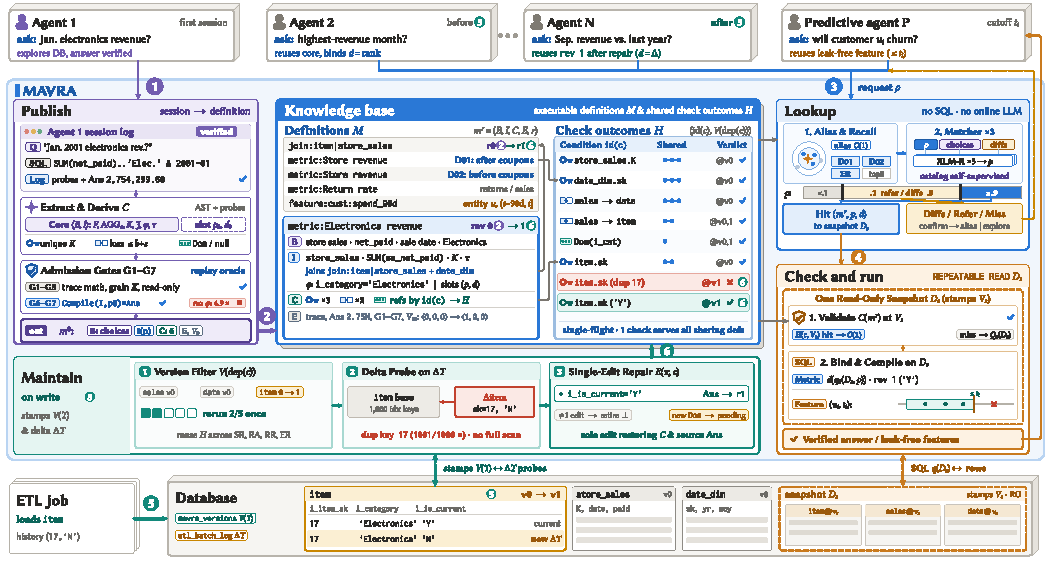
\includegraphics[width=\textwidth,trim=0 0.2mm 0 0.6mm,clip]{figures/architecture}%
\caption{\bt{Components of \system{} around one shared knowledge base, and the path of one definition through them: publication (steps 1--2), lookup and reuse (3--4), and maintenance after a write (5--6). Small circled numbers mark the step that wrote a state.}{\system{} 围绕一个共享知识库的各组件，以及一个定义经过它们的路径：发布（步骤 1--2）、查找与复用（3--4）、写入后的维护（5--6）。小圆圈数字标出写入该状态的步骤。}}
\label{fig:architecture}
\Description{Agents 1, 2, N and predictive agent P sit above MAVRA; the database and an ETL job sit below it. Inside MAVRA, five components surround a knowledge base. Publish, on the left, takes Agent 1's verified session (the SQL with the filter i_category = 'Electronics' marked as phi and the period d_year = 2001 AND d_moy = 1 marked as parameter p, the probes, and the answer 2,754,299.60), extracts the implementation I and parameter p0 with an LLM, derives conditions C (keys unique, join coverage within b plus epsilon, domain and null bounds from probes) without an LLM, and passes gates G1 to G7; replaying on the learning tables shows that Compile(I, p0) equals the answer while a draft without phi is 4.9 times larger and is rejected. Its output, revision 0, enters the knowledge base (step 2). The knowledge base is one key-value store shared by all agents. Definitions are entries keyed by kind and name, one per revision m^r = (B, I, C, E, r): join:item|store_sales, two metric:Store revenue entries (D01 after coupons, D02 before coupons), metric:Return rate, feature:customer:spend_90d, and the expanded metric:Electronics revenue, whose joins reference the join entry by key and whose conditions reference outcomes in H by signature. The lookup state holds aliases (store turnover maps to D01 and D02), one vector per entry, and three judges trained on the catalog. Check outcomes H are keyed by (id(c), V(dep(c))): date_dim at version 0 passes and serves three definitions; store_sales to date_dim at version 0 passes; item at version 0 passes; item at version 1 fails and item with 'Y' at version 1 passes, both written in step 6. Lookup, on the right, receives requests (step 3), reads the alias table, recalls the 8 nearest definitions with bge-m3, scores them with three cross-encoder judges, and decides with thresholds 0.1 and 0.9; replies are hit, same name with differences, refer (a confirmed reference becomes an alias), or miss. A hit with m, p, d goes to Check and run (step 4), which checks C against outcomes in H at the snapshot's versions, runs the compiled query in one snapshot, compiles features per entity and cutoff, and returns the answer to the agent. At the bottom, the ETL job loads an item history row for key 17 (step 5). Maintain stamps versions V(T), Stage 1 skips conditions whose tables kept their versions and reruns 2 of 5 checks once for all definitions, Stage 2 checks only the inserted rows and finds key 17 twice, and Repair keeps a sole single edit that preserves the answer, i_is_current = 'Y', publishing revision 1 with outcomes at the new versions (step 6); otherwise it retires the definition or marks it pending. Thin arrows are calls, thick arrows write shared state, grey arrows are references by key or reads of the knowledge base, and dashed arrows read database state.}
\end{figure*}

\subsection{\bt{Knowledge Base}{知识库}}
\label{sec:knowledge-base}
\bi{To separate invariant business logic from changing table data, the knowledge base keeps two persistent key--value stores (Figure~\ref{fig:architecture}, center):
(1)~\emph{Definitions} $M$ store catalog entries under typed keys (\code{metric:}, \code{feature:}, and \code{join:}). Each metric entry holds a versioned tuple $m^r=(B,I,C,E,r)$ (Section~\ref{sec:shared-object})---business choices~$B$, compact relational implementation~$I$ (${\sim}0.6$\,KB), derived checks~$C(I)$, provenance~$E$, and revision~$r$---while each feature entry $f^r$ adds an entity mapping and look-back window (Section~\ref{sec:features}). Entries reference shared \code{join:} records by key rather than copying SQL, and keep same-name metrics with different formulas as separate entries (such as \code{D01} after-coupon vs.\ \code{D02} before-coupon \emph{store revenue} in Figure~\ref{fig:architecture}).
(2)~\emph{Check outcomes} $\mathcal H$ cache validation verdicts by $(\operatorname{id}(c), V(\operatorname{dep}(c)))$ (Section~\ref{sec:maintenance}). Because $\mathcal H$ is keyed by check signature and table version stamps, a single check (e.g., on \code{date\_dim}) serves every definition that references it, and new writes simply append new stamped verdicts without overwriting older snapshots.}
{为将不变业务逻辑与动态表数据分离，知识库维护两类持久化键值存储（图~\ref{fig:architecture} 中部）：
（1）\emph{定义库} $M$ 按类型前缀键（\code{metric:}、\code{feature:} 与 \code{join:}）组织目录。每条指标保存版本化元组 $m^r=(B,I,C,E,r)$（第~\ref{sec:shared-object} 节，含业务口径~$B$、约 $0.6$\,KB 的紧凑关系实现~$I$、派生检查~$C(I)$、溯源证据~$E$ 与修订号~$r$），特征条目 $f^r$ 另含实体映射与回看窗口（第~\ref{sec:features} 节）。条目按键引用共享 \code{join:} 记录而不复制 SQL，并将同名异义指标存为独立条目（如图~\ref{fig:architecture} 中扣券后 \code{D01} 与扣券前 \code{D02} 两条\emph{门店营业额}）。
（2）\emph{检查结论库} $\mathcal H$ 按 $(\operatorname{id}(c), V(\operatorname{dep}(c)))$ 缓存验证判定（第~\ref{sec:maintenance} 节）。由于以条件签名加表版本戳为键，单次检查（如 \code{date\_dim} 主键检查）可供所有引用它的定义共用，新写入仅追加新版本记录而不覆盖旧快照。}

\subsection{\bt{Components and End-to-End Workflow}{核心组件与端到端流程}}
\label{sec:components}
\bi{Figure~\ref{fig:architecture} traces one definition across its full lifecycle in six steps.
In \emph{Publish (steps 1--2, left)}, Agent~1 finishes a verified session for January 2001 electronics revenue ($2{,}754{,}299.60$; step~1). \emph{Publish} traces the arithmetic chain behind that answer without sending raw rows to an LLM, factors January 2001 into parameter slot $p_0$, derives choices $B$ and checks $C(I)$ from $I$, and compiles fresh SQL from $I$ to pass gates G1--G7 before writing \code{metric:Electronics revenue} ($r=0$) and its $\mathcal H$ verdicts (step~2; Section~\ref{sec:publication}).}
{图~\ref{fig:architecture} 用六个步骤展示了一份定义的完整生命周期。
在\emph{发布（步骤 1--2，左）}中，智能体~1 完成 2001 年 1 月电子商品营业额的核验会话（$2{,}754{,}299.60$；步骤~1）。\emph{发布}组件在不向大模型发送原始行的前提下追踪答案算术链，将 2001 年 1 月剥离为参数槽 $p_0$，从 $I$ 导出 $B$ 与 $C(I)$，并仅凭 $I$ 编译新 SQL 通过 G1--G7 后写入 \code{metric:Electronics revenue}（$r=0$）及其 $\mathcal H$ 结论（步骤~2；第~\ref{sec:publication} 节）。}

\bi{In \emph{Lookup and Check-and-run (steps 3--4, right)}, Agent~2 asks for the highest-revenue month. \emph{Lookup} checks the alias table, recalls top-$K$ candidates via embeddings on a miss, and scores choice consistency with local cross-encoders---resolving \code{Electronics revenue} with monthly ranking $d$ without writing SQL or calling an LLM (or returning competing diffs when a choice stays open; step~3, Section~\ref{sec:lookup}). \emph{Check and run} then opens one read-only snapshot $D_s$, verifies $C(m^r)$ at stamps $V_s$ through $\mathcal H$, and runs the compiled query on $D_s$ with zero exploration (step~4).}
{在\emph{查找与检查执行（步骤 3--4，右）}中，智能体~2 查询最高营业额月份。\emph{查找}先查别名表，未命中则向量召回 top-$K$ 候选并由本地交叉编码器打分，免写 SQL、免调大模型选定 \code{Electronics revenue} 及月度排名 $d$（口径开放时返回竞争差异；步骤~3，第~\ref{sec:lookup} 节）。随后\emph{检查并执行}开启单一只读快照 $D_s$，在版本戳 $V_s$ 下经 $\mathcal H$ 校验 $C(m^r)$ 并直接执行编译查询，全程零探查（步骤~4）。}

\bi{In \emph{Maintain (steps 5--6, bottom)}, an ETL load appends historical \code{item} rows, advancing $V(\code{item})$ and duplicating \code{item\_id=17} (step~5). \emph{Maintain} reuses unchanged \code{date\_dim} verdicts in $\mathcal H$, probes only inserted rows $\Delta T$ on \code{item}, and admits the unique single-edit fix \code{i\_is\_current='Y'} after checking that it restores uniqueness, reproduces Agent~1's source answer, and leaves untouched history unchanged---publishing revision~1 (step~6, Section~\ref{sec:maintenance}). Agent~$N$ then reuses revision~1 for September year-over-year revenue without double-counting, while predictive agent~P reuses leak-free feature \code{spend\_90d} over the same $\mathcal H$.}
{在\emph{维护（步骤 5--6，下）}中，ETL 作业追加 \code{item} 历史行，推进 $V(\code{item})$ 并导致 \code{item\_id=17} 重复（步骤~5）。\emph{维护}复用 $\mathcal H$ 中未变的 \code{date\_dim} 结论，仅在新增行 $\Delta T$ 上探测 \code{item}，确认唯一单步补丁 \code{i\_is\_current='Y'} 恢复唯一性、复现源答案且不改未变历史后发布修订版~1（步骤~6，第~\ref{sec:maintenance} 节）。此后智能体~$N$ 直接复用修订版~1 算准 9 月同比，预测智能体~P 也共享 $\mathcal H$ 复用防泄漏特征 \code{spend\_90d}。}
